\documentclass{article}
\usepackage{amsmath}
\usepackage{tikz}
\usepackage{amsfonts}
\usepackage{graphicx}
\usepackage{algorithm}
\usepackage{algpseudocode}
\usepackage[toc,page]{appendix}
\usetikzlibrary{positioning}
\begin{document}

\title {consensus seminar}
\author {ertosns}
\date {2023/6/7}
\maketitle

\section{ Overview}

The DarkFi blockchain is  proof of stake  privacy focused, with high incentive monetary policy.

\subsection{ Blockchain}

 Blockchain $\mathbb{C_{loc}}$ is a series of epochs: it's a tree of chains,
$C^1$, $C^2$, $\dots$, $C^n$, the chain ending in a single leader per slot signals finalization.


Each participant stores it's own local view of the Blockchain $C_{loc}$ is a sequence of blocks $B_i$ (i>0), where each $B \in C_{loc}$
$$ B = (tx_{lead},st)$$
$$tx_{lead} = (LEAD, header, txs, stx_{proof})$$
LEAD is a magic word, header is a metadata, and txs is a vector of transaction hash
$stx_{proof}=(cm_{\prime{c}},sn_c,ep,sl,\rho,h,\pi)$
the Block's st is the block data, and h is the hash of that data.
the commitment of the newly created coin is:
$(cm_{c_2},r_{c_2})=COMM(pk^{COIN}||\tau||v_c||\rho_{c_2})$,
$\tau$ is slot timestamp, or index. $sn_c$ is the coin's serial number revealed to spend the coin.
$$sn_c=PRF_{root_{sk}^{COIN}}^{sn}(\rho_c)$$


\subsection{ st transactions}
the blockchain view is a chain of blocks, each block $B_j=(tx_{lead},st)$, while $st$ being the merkle tree structure of the validated transactions received through the network, that money transfer, and lead transactions.

\subsection{ LEAD statement}
for $x=(cm_{c_2},sn_{c_1},\eta,sl,\rho,h,ptr,\mu_{\rho},\mu_{y},root)$, and
\newline
$w=(path,root_{sk^{COIN}},path_{sk^{COIN}},\tau_c,\rho_c,r_{c_1},v,r_{c_2})$
for tuple $(x,w) \in L_{lead}$ iff:

 \item $pk^{COIN} = PRF_{root_{sk}^{COIN}}^{pk}(\tau_c)$.
 \item $\rho_{c_2}=PRF_{root_{sk_{c_1}}^{COIN}}^{evl}(\rho_{c_1})$.
 note here the nonce of the new coin is deterministically driven from the nonce of the old coin, this works as resistance mechanism to allow the same coin to be eligible for leadership more than once in the same epoch.
 \item $\forall i \in \{1,2\} : DeComm(cm_{c_i},pk^{COIN}||v||\rho_{c_i},r_{c_i})=T$.
 \item path is a valid Merkle tree path to $cm_{c_1}$ in the tree with the root root.
 \item $path_{sk^{COIN}}$ is a valid path to a leaf at position $sl-\tau_c$ in a tree with a root $root_{sk}^{COIN}$.
 \item $sn_{c_1}= PRF_{root_{sk}^{COIN}}^{sn}(\rho_{c_1})$
 \item $y = \mu_{y}^{root_{sk_{c_1}}^{COIN}||\rho_c}$
 \item $\rho = \mu_{\rho}^{root_{sk_{c_1}}^{COIN}||\rho_c}$,

 \item $y< T(v)$

   $\rho$ id randomness from $\eta$.  $\pi$ is the NIZK proof of the LEAD statement.
   note! that this process involves burning old coin $c_1$, minting new  $c_2$ of the same value + reward.


\subsubsection{ validation rules}

validation of proposed lead proof as follows:
\begin{itemize}
\item slot index is less than current slot index, epoch index is less than or equal current epoch index.
\item proposal extend from valid fork chain
\item proposal extend highest ranking block (see \ref{finalization})
\item transactions doesn't exceed max limit
\item signature is valid based off producer public key
\item verify block hash
\item verify previous block hash
\item public inputs $\mu_y$, $\mu_{rho}$ are derived from on-chain VRF output $\eta$, and current slot, and block producer signature, and public key.
\item public inputs of target 2-term approximations $\sigma_1$, $\sigma_2$ are valid given total network stake and controller parameters
\item the competing coin nullifier isn't published before to protect against double spening, before burning the coin.
\item burnt coin's commitment rooted by commitments merkle tree root.
\item verify block transactions

\end{itemize}

\subsection{ Epoch}

An epoch is a vector of blocks. Some of the  blocks might be empty if there is no winnig leader. tokens in stake are constant during the epoch.

\subsection{ Leader selection}

At the onset of each slot each stakeholder needs to verify if it's
the weighted random leader for this slot.

$$y < T_{i}$$ check if the random y output is less than some
threshold

This statement might hold true for zero or more stakeholders, thus
we might end up with multiple leaders for a slot, and other times no
leader. Also note that no node would know the leader identity or how many
leaders are there for the slot, until it receives a signed block with
a proof claiming to be a leader.


$\textbf{sid}$ is block id

$$\phi_{f} = 1 - (1-f)^{\alpha_i}$$ $$T_{i} =
L \phi_{f}(\alpha_i^j)$$

Note that $\phi_f(1)=f$, $\textbf{f}$: the active slot coefficient is
the probability that a party holding all the stake will be selected to be
a leader. Stakeholder is selected as leader for slot j with probability
$\phi_f(\alpha_i)$, $\alpha_i$ is $U_i$ relative stake.


\subsection{ automating f tuning}

the stable consensus token supply is maintained by the help of discrete PID controller, that maintain stabilized occurance of single leader per slot.

\subsubsection{ control lottery f tunning paramter }

$$f[k] = f[k-1] + K_1e[k] + K_2e[k-1] + K_3e[k-2]$$

with $k_1 = k_p + K_i + K_d$,  $k_2 = -K_p -2K_d$,  $k_3 = K_d$, and e is the error function.


\subsection{ target T n-term approximation }
target function is approximated to avoid use of power, and division in zk, since no function in the family of functions that have independent aggregation property achieve avoid it (see appendix).

\subsubsection{ target function}

 target fuction T: $$ T = L * \phi(\sigma) = L * (1- (1 - f)^{\sigma}) $$
 $\sigma$ is relative stake.
 f is tuning parameter, or the probability of winning have all the stake
 L is field length

\subsection{ $\phi(\sigma)$ approximation}

 $$\phi(\sigma) = 1 - (1-f)^{\sigma} $$
 $$ = 1 - e^{\sigma ln(1-f)} $$
 $$ = 1 - (1 + \sum_{n=1}^{\infty}\frac{(\sigma ln (1-f))^n}{n!}) $$
 $$ \sigma = \frac{s}{\Sigma} $$
 s is stake, and $\Sigma$ is total stake.

\subsubsection{ target T n term approximation}

 $$ k = L ln (1-f)^1 $$
 $$ k^{'n} =  L ln (1-f)^n $$
 $$ T = -[k\sigma + \frac{k^{''}}{2!} \sigma^2 + \dots +\frac{ k^{'n}}{n!}\sigma^n] $$
 $$  = -[\frac{k}{\Sigma}s + \frac{k^{''}}{\Sigma^2 2!} s^2 + \dots +\frac{k^{'n}}{\Sigma^n n!} s^n] $$

\subsubsection{ comparison of original target to approximation }

\begin{figure}
  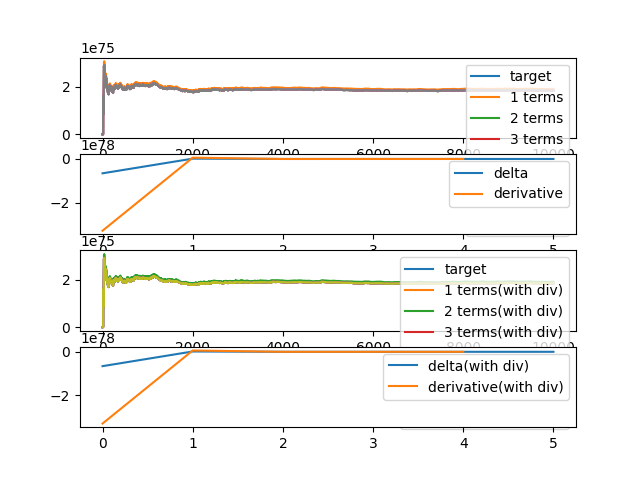
\includegraphics{target.png}
  \caption{approximation comparison to the original }
\end{figure}



\subsection {Linear family functions}

In the previous leader selection function, it has the unique
property of independent aggregation of the stakes, meaning the
property of a leader winning leadership with stakes $\sigma$
is independent of whether the stakeholder would act as a pool
of stakes, or distributed stakes on competing coins.  "one minus
the probability" of winning leadership with aggregated stakes is
$1-\phi(\sum_{i}\sigma_i)=1-(1+(1-f)^{\sigma_i})=-(1-f)^{\sum_{i}\sigma_i}$,
the joint "one minus probability" of all the stakes (each with
probability $\phi(\sigma_i))$ winning aggregated winning the leadership
$\prod_{i}^{n}(1-\phi(\sigma_i))=-(1-f)^{\sum_i(\sigma_i)}$ thus: $$
1-\phi(\sum_{i}\sigma_i) =\prod_{i}^{n}(1-\phi(\sigma_i)) $$

A non-exponential  linear leader selection can be:

$$y < T $$ $$y = 2^lk \mid 0 \le k \le 1$$ $$T = 2^l\phi(v)$$ $$
\phi(v)=\frac{1}{v_{max+}+c}v  \mid c \in \mathbb{Z}$$

\subsubsection{ Dependent aggregation}

Linear leader selection has the dependent aggregation property, meaning
it's favorable to compete in pools with sum of the stakes over aggregated
stakes of distributed stakes:

$$\phi(\sum_{i}{\sigma_i})>\prod_{i}^{n}{\sigma_i}$$
$$\sum_{i}{\sigma_i}>(\frac{1}{v_{max}+c})^{n-1}v_1v_2 \dots
v_n$$ let's assume the stakes are divided to stakes of value
$\sigma_i=1$ for $\Sigma>1 \in \mathbb{Z}$, $\sum_{i}{\sigma_i}=V$
$$V>(\frac{1}{v_{max}+c})^{n-1}$$ note that $(\frac{1}{v_{max}+c})^{n-1}
< 1, V>1$, thus competing with single coin of the sum of stakes held by
the stakeholder is favorable.

\subsubsection{ Scalar linear aggregation dependent leader selection}

A target function T with scalar coefficients can be formalized as
$$T=2^lk\phi(\Sigma)=2^l(\frac{1}{v_{max}+c})\Sigma$$ let's assume
$v_{max}=2^v$, and $c=0$ then: $$T=2^lk\phi(\Sigma)=2^{l-v}\Sigma$$
then the lead statement is $$y<2^{l-v}\Sigma$$ for example for a group
order or l=    24 bits, and maximum value of $v_{max}=2^{10}$, then
lead statement: $$y<2^{14}\Sigma$$

\subsubsection{ Competing max value coins}

For a stakeholder with $nv_{max}$ absolute stake, $\mid n \in \mathbb{Z}$
it's advantageous for the stakeholder to distribute stakes on $n$
competing coins.

\subsubsection{ Inverse functions}

Inverse lead selection functions doesn't require maximum stake, most
suitable for absolute stake, it has the disadvantage that it's inflating
with increasing rate as time goes on, but it can be function of the
inverse of the slot to control the increasing frequency of winning
leadership.

\subsubsection{ Leader selection without maximum stake upper limit}

The inverse leader selection without maximum stake value can be
$\phi(v)=\frac{v}{v+c} \mid c  > 1$ and inversely proportional
with probability of winning leadership, let it be called leadership
coefficient.


\subsubsection{ Decaying linear leader selection}

As the time goes one, and stakes increase, this means the combined stakes
of all stakeholders increases the probability of winning leadership
in next slots leading to more leaders at a single slot, to maintain,
or to be more general to control this frequency of leaders per slot, c
(the leadership coefficient) need to be function of the slot $sl$, i.e
$c(sl) = \frac{sl}{R}$ where $R$ is epoch size (number of slots in epoch).

\subsubsection{ Pairing leader selection independent aggregation function}

The only family of functions $\phi(\alpha)$ that are isomorphic
to summation on multiplication $\phi(\alpha_1+\alpha_2)
= \phi(\alpha_1)\phi(\alpha_2)$(having the independent aggregation
property) is the exponential function, and since it's impossible to
implement in plonk,  a re-formalization of the lead statement using
pairing that is isomorphic to summation on multiplication is an option.

Let's assume $\phi$ is isomorphic function
between multiplication and addition, $\phi(\alpha) =
\phi(\frac{\alpha}{2})\phi(\frac{\alpha}{2})=\phi(\frac{\alpha}{2})^2$,
thus:
$$\phi(\alpha)=\underbrace{\phi(1)\dots\phi(1)}_\text{$\alpha$}=\phi(1)^\alpha$$
then the only family of functions $\phi : \mathbb{R} \rightarrow
\mathbb{R}$ satisfying this is the exponential function
$$\phi(\alpha)=c^{\alpha} \mid c  \in \mathbb{R}$$

\subsubsection{ no solution for the lead statement parameters, and constants $S,f, \alpha$ defined over group of integers.}

assume there is a solution for the lead statement parameters and constants $S, f, \alpha$ defined over group of integers.
for the statement $y<T$, $$T=L\phi_{max}\phi(\alpha)=S\phi(\alpha)$$
$$S=ord(G)\phi_{max}\phi(\alpha)$$
such that S $in Z$
$\phi_{max}=\phi(\alpha_{max})$ where $\alpha_{max}$ is the maximum stake value being $2^{64}$, following from the previous proof that the family of function haveing independent aggregation property is the exponential function $f^\alpha$, and $f \in Z | f>1$, the smallest value satisfying f is $f=2$, then $$\phi_{max} = 2^{2^{64}}$$
note that since $ord(G)<<\phi_{max}$ thus $S<<1$, contradiction.


\subsubsection{ Leaky non-resettable beacon}

Built on top of globally synchronized clock, that leaks the nonce $\eta$
of the next epoch a head of time (thus called leaky), non-resettable
in the sense that the random nonce is deterministic at slot s, while
assuring security against adversary controlling some stakeholders.

For an epoch j, the nonce $\eta_j$ is calculated by hash function H, as:

$$\eta_j = H(\eta_{j-1}||j||v)$$

v is the concatenation of the value $\rho$ in all blocks from the
beginning of epoch $e_{i-1}$ to the slot with timestamp up to $(j-2)R +
\frac{16k}{1+\epsilon}$, note that k is a persistence security parameter,
R is the epoch length in terms of slots.

\subsection {toward better decentralization in ouroboros}

the randomization of the leader selection at each slot is hinged on the random $y$, $\mu_y$, $\rho_c$, those three values are dervied from $\eta$, and root of the secret keys, the root of the secret keys for each stakeholder can be sampled, and derived beforehand, but $\eta$ is a response to global random oracle query, so it's security is hinged on $\textit{centralized global random node}$.

\subsubsection{ solution}

to break this centeralization, a decentralized emulation of $G_{ro}$ functionality for calculation of: $\eta_i=PRF^{G_{ro}}_{\eta_{i-1}}(\psi)$
$$\psi   =  hash(tx^{ep}_{0})$$
$$\eta_0 =  hash(\mathrm{"let\; there\; be\; dark!"})$$
note that first transaction in the block, is the proof transaction.

%\section {stake&unstake}

\section {on-chain true random oracle}

\subsection{democratized random lottery seed}
at slot i, randomness $\eta_i$ in the $y$ variable in the leader election comparison, is the output of VRF.
$$\eta_i=VRF(coin_{sk}, \eta_{i-1}||slot_{i})$$  which is publicly verifiable through $verify(\eta_{i-1}||slot_{id}, coin_{pk})$, where $coin_{pk}$ is constrained as public input, and keypair $(coin_{sk},coin_{pk})$ is protected against grinding attack by published nullifier in the same contract, has advantage over ouroboros, which reduce the grinding effect through multiple queries for the random oracle for favoring high probability of winning by limiting the number of queries to the random oracle.  \cite{ouroboros_genesis}

\subsection {grinding $\eta$, and delayed stake contract}
although randomness from the lead stakeholder provider is decentralized, doesn't reveal identity of the provider, more robust than limited access global random oracle, it's deterministic, predictable, meaning, even with time-locked contracts (see \ref{timelocked}), there is a window between un-stake, and stake contracts, or for new adversarial stakeholder, it's possible to target winning at $slot_{id}$, by trying different key pairs, and picking secret key corresponding with lowest \emph{y} possible.
that attack can be prevented by delaying reward proposals from newly staked coins by N slots, N be at least 1, N being a security parameter.

\subsection {omerta attack}
although selecting key pairs corresponding of $\eta$ with lowest corresponding $y$ using public on-chain data is fixed, it's still possible to make off-chain agreements, for example at slot i if the contract execution is delayed N slots, it's possible through N agreements with winners of slots \emph{i} to \emph{i+N}, and since calculation of $\eta$ is predictable, it's possible to pick elect key pair corresponding to lowest \emph{y} at slot i+N+1 in the future, early at i slot.
note that the off-chain agreement is done with probabilistic winners, but once this attack is done once (even if possible with low probability), the adversaries will have high leverage on winning, by mining lowest possible \emph{y}.

the attack can be fixed, by introducing unpredictable random parameter: $$\eta_i = VRF(coin_{sk}, \eta_{i-1}||hash(block_{i-2})||slot_i)$$


note! secret key is constrained 1 slot ahead (assume $N=1$ for simplicity), and grinding isn't possible since the staked coin is restricted from reward proposals for 1 slot, and $\eta_{i-1}$ isn't known yet, omerta attack isn't possible since $hash(block_{i-2}))$ isn't known ahead of time, also $\eta_{i-1}$, and $hash(block_{i-2})$ are phased out to prevent lead at slot \emph{i-1} from grinding $hash(block_{i-1})$  through different transactions permutations.

\subsection {perpetual lead with predictable block hash}


slots are divided into N+2 cycles, (N is security parameter $N \ge 1$), adversary assume winning lottery in the consecutive slots i to i+N, with certain probability, then winning leadership at slot i+N+1 becomes highly probable, only the first block at slot i include a single stake transaction (note staked DRK execution is delayed to slot i+N+1), rest of blocks i+1 to i+N are left with empty transactions, then predicting $\eta_i$ to $\eta_{i+N+1}$ is possible, and thus grinding attack can be executed.

\begin{figure}
  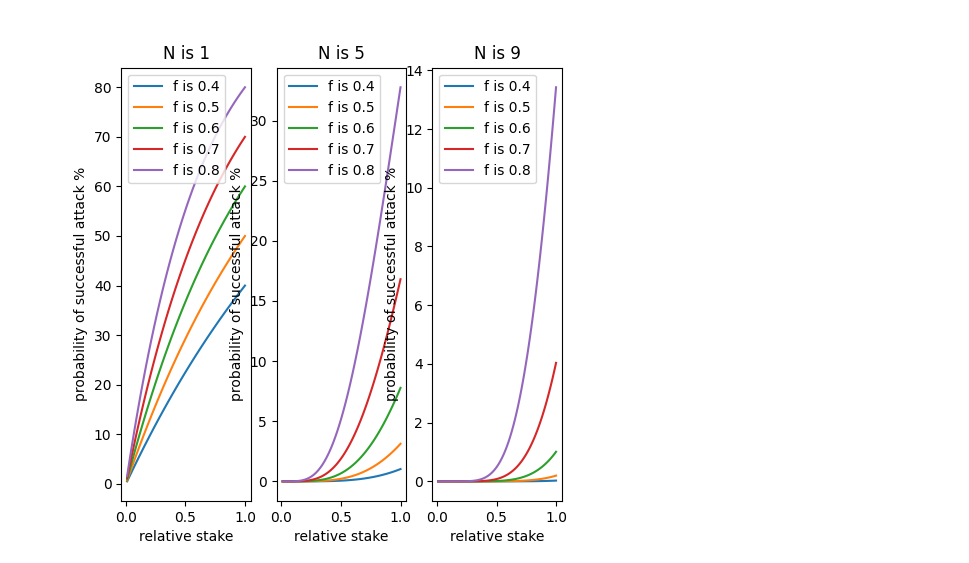
\includegraphics[scale=0.8,left]{prob.png}
  \caption{probability of attack for different security parameter }
\end{figure}


if we plot that probability of successful attack, for N (security parameter) delayed slots, function of relative stake (see figure 1), from graph we  note that even with 100% of stake,  assuming average secondary controller output f is 0.6 (simulation shows close results), then the probability of successful attack is ~ 1%, for 60% staked ratio, and f is 0.6 probability of successful attack is close to zero.

\subsection {conclusion}
the omerta attack with perpetual lead is of diminishing probability of success for security parameter $N \ge 9$.

\section{chain fork}
fork can occur when multiple stakeholders publish proposal for valid proof of leadership.
winning stakeholder can choose to fork with a new block, extend a chain, or extend chanonical longest chain.

\subsection{fork finalization}
finalization is a compound of longest chain, and single leadership frequency, at the end of any slot, finalization, and re-syncing happen when there is single leader per slot, single leader frequency is controller with secondary discrete PID controller in cascade control.
such mechanism is resilient to bribery attack \cite{attack_bribery}, and NAS attack (when the stakeholder write a transaction in one chain, and rewrite the transaction in parallel chain of equivalent stake, and equal fork depth, using relatively small stake) since probability of winning leadership with single leader frequency at small stake at more than one slot during the fork depth  is of negligible probability.
% TODO exercise what is length of the fork to win two slots for example for someone with even 1,5,10% of stake.

\subsection {finalization degree of freedom}
it's possible for single lead stakeholder at the end of a fork to honor certain fork chain based off off-chain agreement, or if the stake stakeholder leads another block in the fork.

\label{finalization}
\subsection {deterministic finalization}
if there are multiple chain fork, execute \emph{rank} function on the longest chains, leadership assigned to the highest rank, and block is finalized.

note that same rank collision is of negligible probability, but in such case, the stakeholder can choose either of which if there is such collision between highest ranks.


\begin{algorithm}
\caption{rank}\label{alg:cap}
\begin{algorithmic}

\State $pks \gets \textbf{list of fork competing coin's pks}$
\State $\eta \gets random()$ \Comment{output of on-chain VRF}
\State $N \gets len(pks)$
\State $orders \gets []$
%\State $N \gets n$
\While{$N \neq 0$}
\State $pk \gets pks[N]$
\State $order \gets pk \% (\eta >> 3) $
\State $N \gets N-1$
\State $orders.append((pk,order))$
\EndWhile
\State \Return orders
\end{algorithmic}
\end{algorithm}


\subsection {instant finality}
the single leader controller aka the secondary controller responsible for fork finalization through single lead per slot achieve 30-38\% accuracy on the simulation \cite{lotterysim}, and up to 50\% accuracy on test-net (increases over time; seams the controller learn to adapt pretty well; difference between simulation, and test-net is the distribution of random variables, simulation assumes uniform distribution, which seams to not be the case).
instant finality through 100\% secondary controller accuracy can be achieved through \emph{L2} leadership election chain \cite{khonsu}, meanwhile deterministic finalization(see \ref{finalization}) already achieves instant finality, since highest order rank in multiple leaders per block resolves the fork, although it's subject to long rang attack (see \ref{longrange})


\label{longrange}
\subsection {long range attack}
offline stakeholder can be malicious if won leadership with highest rank without synchronization, or due to network level corruption by malicious attacker that lead to same case of out of sync chains, if stakeholder came online of sudden and propose different chain with highest ranking leadership proof than canonical one, then transaction can be rewritten by validators discarding established chain, and extending proposed chain.


\subsubsection {mitigating long range attack: posterior corruption}
\item extending only long chains filters out short chains
\item forking parallel chain requires $\gt 50\%$ of staked DRK and has success rate $$ (1-(1-f)^{\sigma})^{L} $$
  \emph{L} is fork length, $\sigma$ is relative stake, \emph{f} is probability of winning lottery owning all the stake, from test-net, and simulation $f$ tend to be around 0.6, note that if fork length is 1 then validators choose between highest rank, so lowest possible fork length to rewrite transactions is 2, then at 50\%  of stake to take pessimistic point of view at $f=0.6$ probability of such attack is $((1-(1-0.6)^{0.5})^2w=0.135$ assuming malicious attacker always gets highest rank, which is random process (assuming independent Event), happen at probability $F^L $ ,F being number of fork, lowest possible is $F=2$ meanwhile probability of attack at $f=0.6$ with BFT performance 33\% of stake is assumed malicious at lowest possible fork length is $(1-(1-0.6)^{0.33})^2=0.068$ assuming malicious attacker always get highest rank, and probability of getting sequence of high ranks is $F^L$, assume the lowest possible number of forks $F=2$ (which is very pessimistic, F is proportional to number of stakeholders) then the successful attack at $33\%$ stake, $f=0.6$, $F=2$, and $L=2$ have probability of $\frac{0.068}{F^L} = 0.017$, since the fork happen with probability = 1 - $\emph{ accuracy of single lead}$ = $1-acc$, assuming it happens at random, then probability of Long range attack $P_{L=2}(\emph{LRA})$ = $\frac{(1-(1-f)^{\sigma})(1-acc)}{F}^L = 0.00764$.

  \label{longrangefig}
  \begin{figure}
    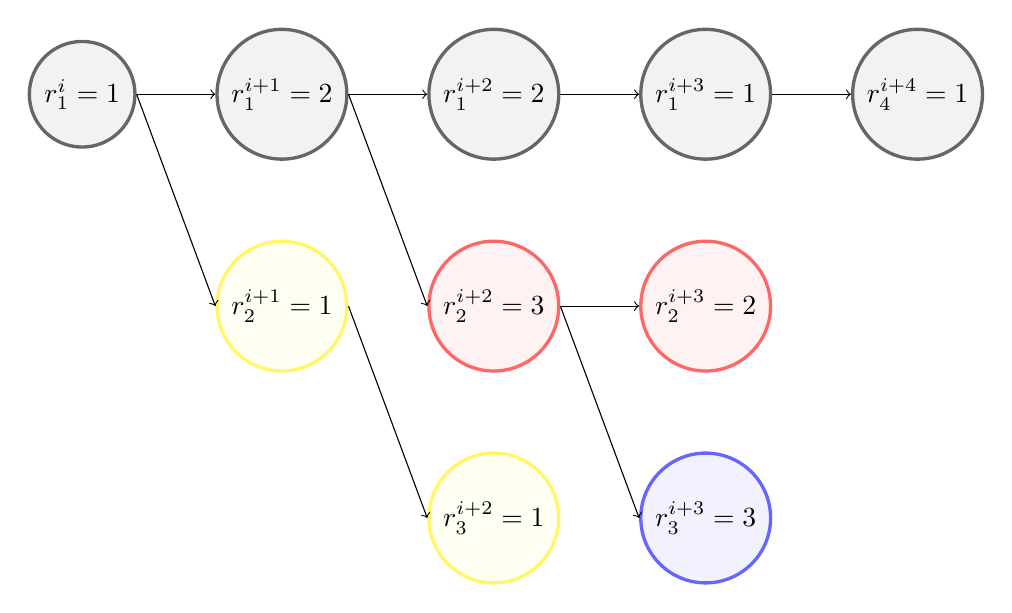
\begin{tikzpicture}
      [
        roundb/.style={circle, draw=black!60, fill=black!5, very thick, minimum size=5mm},
        roundr/.style={circle, draw=red!60, fill=red!5, very thick, minimum size=5mm},
        roundg/.style={circle, draw=green!60, fill=green!5, very thick, minimum size=5mm},
        roundu/.style={circle, draw=blue!60, fill=blue!5, very thick, minimum size=5mm},
        roundy/.style={circle, draw=yellow!60, fill=yellow!5, very thick, minimum size=5mm}
      ]
      \node[roundb] (r) {$r^{i}_1=1$};
      \node[roundb] (r11) [right=of r] {$r^{i+1}_1=2$};
      \node[roundy] (r12) [below=of r11] {$r^{i+1}_2=1$};
      \node[roundb] (r21) [right=of r11] {$r^{i+2}_1=2$};
      \node[roundr] (r22) [below=of r21] {$r^{i+2}_2=3$};
      \node[roundy] (r23) [below=of r22] {$r^{i+2}_3=1$};
      \node[roundb] (r31) [right=of r21] {$r^{i+3}_1=1$};
      \node[roundr] (r32) [below=of r31] {$r^{i+3}_2=2$};
      \node[roundu] (r33) [below=of r32] {$r^{i+3}_3=3$};
      \node[roundb] (r41) [right=of r31] {$r^{i+4}_4=1$};
      \draw[->] (r.east) -- (r11.west);
      \draw[->] (r.east) -- (r12.west);
      \draw[->] (r11.east) -- (r21.west);
      \draw[->] (r11.east) -- (r22.west);
      \draw[->] (r12.east) -- (r23.west);
      \draw[->] (r21.east) -- (r31.west);
      \draw[->] (r22.east) -- (r32.west);
      \draw[->] (r22.east) -- (r33.west);
      \draw[->] (r31.east) -- (r41.west);
    \end{tikzpicture}
    \caption{long range attack case study, $r^{i}_{j}=k$ means block at slot \emph{i} of index \emph{j} has rank \emph{k}}
    \end{figure}

\item in span of 4 slots if chain $r^i_1$,$r^{i+1}_2$,$r^{i+2}_3$ came online at slot $i+3$ (see figure \ref{longrangefig}), the attack is possible starting from slot $i+3$, assuming malicious attacker owns $33\%$ (BFT performance) of stake, under same previous parameters, probability of attack is $0.00764$, in other words the possibility of rewriting transactions loaded in blocks $r^{i+1}_1$, $r^{i+2}_2$ by malicious attacker that only sync at slot $i+3$ owning block proofs $r^{i+1}_2,r^{i+2}_3$ owning  33\% of stake at same parameters above is successful once in 130 attempts respectively.

  \subsubsection { costly block creation }

\item unlike different PoS blockchain, the lead proof creation here is costly, it requires stake, and a some luck proportional to owned stake, $P_{L=2}(LRA) \sim 0.00764$, assume diminishing probability of attack at costly block creation is $\lt 1e-6$, $P_{L=6}(LRA) \sim 4.4e-7$, with difference being just \emph{4} slots

\item victims of LRA malicious attacker are new nodes, if they only connect to the malicious attacker, they see attacker's chain, if connected to more nodes, and see a fork, new nodes has to wait for 4 more slots before making a tx.

  \section{slashing}


\section {time frequency}
blockchain lifetime is series of epoch


\subsection {epoch}
multiple slots during which the reward value is fixed, and set by primary controller in the cascade control mechanism \cite{cascade}, and stake is dynamic different from the concept of the epoch in ouroboros, in which the epoch has frozen stake for leadership purposes.

\subsection {slot}
period of time in which new block is issued

\subsection {span}
leader election span of time, which can be unspecified period using controller, or fixed 1/3 of slot as described in khonsu \cite{khonsu} during which leaders for slots in the future are elected.

\section {timelocked contract}
time locked contracts is part of contract, and consensus validation rules, contract locked for \emph{n} epochs is locked by committing to epoch index used in burn proof constrained coin.

\label{timelocked}
\subsection {grinding attack in stake, unstake contracts}
stakeholders can move funds between different accounts during the slot for higher probability of winning, such attack can be prevented via timelocked contracts.


\section {fee mechanism}
slot is clock based, of fixed time length, as a result there is single target of computational cost normal computer (to be defined) can process in a single slot, variable block gas mechanism as in eip1559 won't work.

\subsection{ fixed slot length}
fixed slot length dictates that there is limited amount of computation possible during single slot block gas, or block computational cost is fixed let's call it C, let's distinguish between block computational cost capacity CC, and actual block cost C.

\subsection{fee volatility}
sudden increase/decrease in demand to fixed supply would lead to spikes in fee cost, and it' can't be accommodated for nor maintained increase in demand, such issues are not auction mechanism design issue, but scalability issues that could mitigated through zk rollups, sharding, parallel tx processing, faster consensus protocols, etc.

\subsection{ base fee burning}
burning base fee \emph{b} based off parent blocks computational cost, with two conditions: base fee is based off previous blocks computational cost to avoid malicious attacks from current miner to drive fee up, secondly base fee is deterministically calculated rather than agreement between user, and leader in which collusion can occur off-chain to evade base fee burning.

\subsubsection{ why fee is burned}
reduce inflation, raise DRK value.
increase cost of spamming, and fake transaction.

\subsubsection{ tatonment and control}
eip1559 \cite{eip1559} propose base fee update rule and discovery of market clearing price, and report on the protocol \cite{eip1559_report} propose interpolation of base fee between the two different block gas costs at 12.5M, and 25M for fine grained base fee results.
however due to fixed slot length, and inability to mitigate sudden increase/decrease in demand more fine grain base fee technique is required, that tatonment addressed above is bad approximation of PID controller.

\subsubsubsection{ base fee based off PID control}
 fine grain tatonment can be achieved through PID controller that can reduce spikes in base fee price due to change in demand, with feedback from previous block's cost C.
 for example base fee f at block i is $$ f[i] = f[i-1] + K_1e[i] + K_2 e[i-1] + K_3e[i-2] $$
 where $e[i]$ is error function in previous block i-1, $K_1$, $K_2$, $K_3$ are discrete controller parameters (to be tuned).
 $e[i]$ is the difference between block computation cost capacity, and block cost:
 $$ e[i] = CC[i-1] - C[i-i]$$
 note that block computational cost capacity \emph{CC} has to be slightly lower than actual computational cost \emph{ACC} to enable controller to adapt to high demand, for example CC=0.98ACC.

 \subsection{tip}
 tip is necessary for transactions inclusion in the block by the block lead.

\subsubsection{ tip first price auction}
 tip is similar to eip1559 is a priority fee implemented as first price auction due to simplicity, and undue trusted third party required in more efficient auctions i.e vickery auction.
 client/user, or tx creators propose tx tip \emph{t}, assuming client's fee $ = t+b = $ max cap fee, then auction utility is nonzero, and max cap isn't required to be added by client in tx header, only tx tip is sufficient.

 \subsubsection {tipless fee mechanism}
for better wallet UX, tip auction can be replaced by tip being function of tx computational cost for inclusion in the block, in such cases, all transactions are priced the same per computational unite, but in cases of high demand, lead, and user can collude off-chain to prioritize transactions, other than that, the collusion can't prevent burning fee, or cheating.
note that even if base fee, and tip got low in value due to inflation, it still will not incentivize off-chain collusion, as long as the controller adapts fee to block parent blocks cost \emph{C}

\subsection{ computation unites}
since slots has limited computation unites, computation unites is better suited for fee estimation than gas price based of block size, or type of contract, every dedicated contract call better have some unite of computation for more accurate estimation of cost, otherwise, lead might ditch computationally expensive txs. in that sense, there are two attributes of txs, tips, and computational cost.

\subsection{ delay due to empty slots}
 empty slots with no leads would accumulate pending txs, and would increase base fee on subsequent slots, and users would increase tips for inclusion.



\begin{thebibliography}{999}

\bibitem{ouroboros_genesis}
  Ouroboros Genesis,
  \emph{Composable Proof-of-Stake Blockchains with Dynamic Availability},
  Christian Badertscher, et al,
  22-02-2019

\bibitem{attack_bribery}
  bribery attack,
  \emph{Lecture 18: Bribery and stake grinding attacks},
  David Tse,
  Stanford University, Spring 2020
  04-06-2020

\bibitem{cascade}
  cascade,
  \emph{consensus high incentive monetary policy},
  ertosns,
  15-04-2023

\bibitem{khonsu}
  khonsu,
  \emph{darkfi khonsu consensus},
  ertosns,
  31-12-2022

\bibitem{eip1559}
  eip1559,
  \emph{EIP-1559: Fee market change for ETH 1.0 chain},
  Vitalik Buterin, et al,
  13-04-2019

\bibitem{eip1559_report}
  An Economic Analysis of EIP-1559*,
  \emph{Transaction Fee Mechanism Design for the Ethereum Blockchain},
  tim roughgarden,
  01-12-2020

\bibitem{lotterysim}
  lotterysim,
  \emph{darkfi lottery simulation},
  ertosns,
  11-1-2023
\end{thebibliography}


\end{document}
